%!TEX root = ../thesis.tex
%*******************************************************************************
%*********************************** First Chapter *****************************
%*******************************************************************************
\chapter{Introduction}  %Title of the First Chapter

\ifpdf
    \graphicspath{{Chapter1/Figs/Raster/}{Chapter1/Figs/PDF/}{Chapter1/Figs/}}
\else
    \graphicspath{{Chapter1/Figs/Vector/}{Chapter1/Figs/}}
\fi


%********************************** %First Section  **************************************
\section{Model Construction and Validation} %Section - 1.1 

Creating and validating models for systems (physical and otherwise) is a staple of engineering. It generally entails: 1) designing experiments to gather the most representative available data, 2) creating mathematical representations for the systems, and 3) implementing state and/or parameter estimation in order to improve the accuracy of models using data. It is ideal to perform these steps concurrently. In particular, when model validation is undertaken in an integrated fashion, each step of the validation can be tailored, so that they fit seamlessly together, figure \ref{block_diagram}. Unfortunately, it is rare for this to occur when systems require physical experiments, especially in the context of academia. This is largely because fields involving physical systems, such as vehicles and robotics, were historically in their infancy. Integrated model validation is unfeasible in situations where it is unclear how one would even go about inducing these processes. However, over the past few decades, great fundamental work has been done on both manipulating physical systems, and understanding the general principles that govern their behavior. This has created largely untapped opportunity for high quality modeling and validation. In this work, we perform integrated model validation for electrostatic comb-drive actuators in electrolytes. \\

\begin{figure}[h]
%\begin{minipage}[t]{\linewidth}
    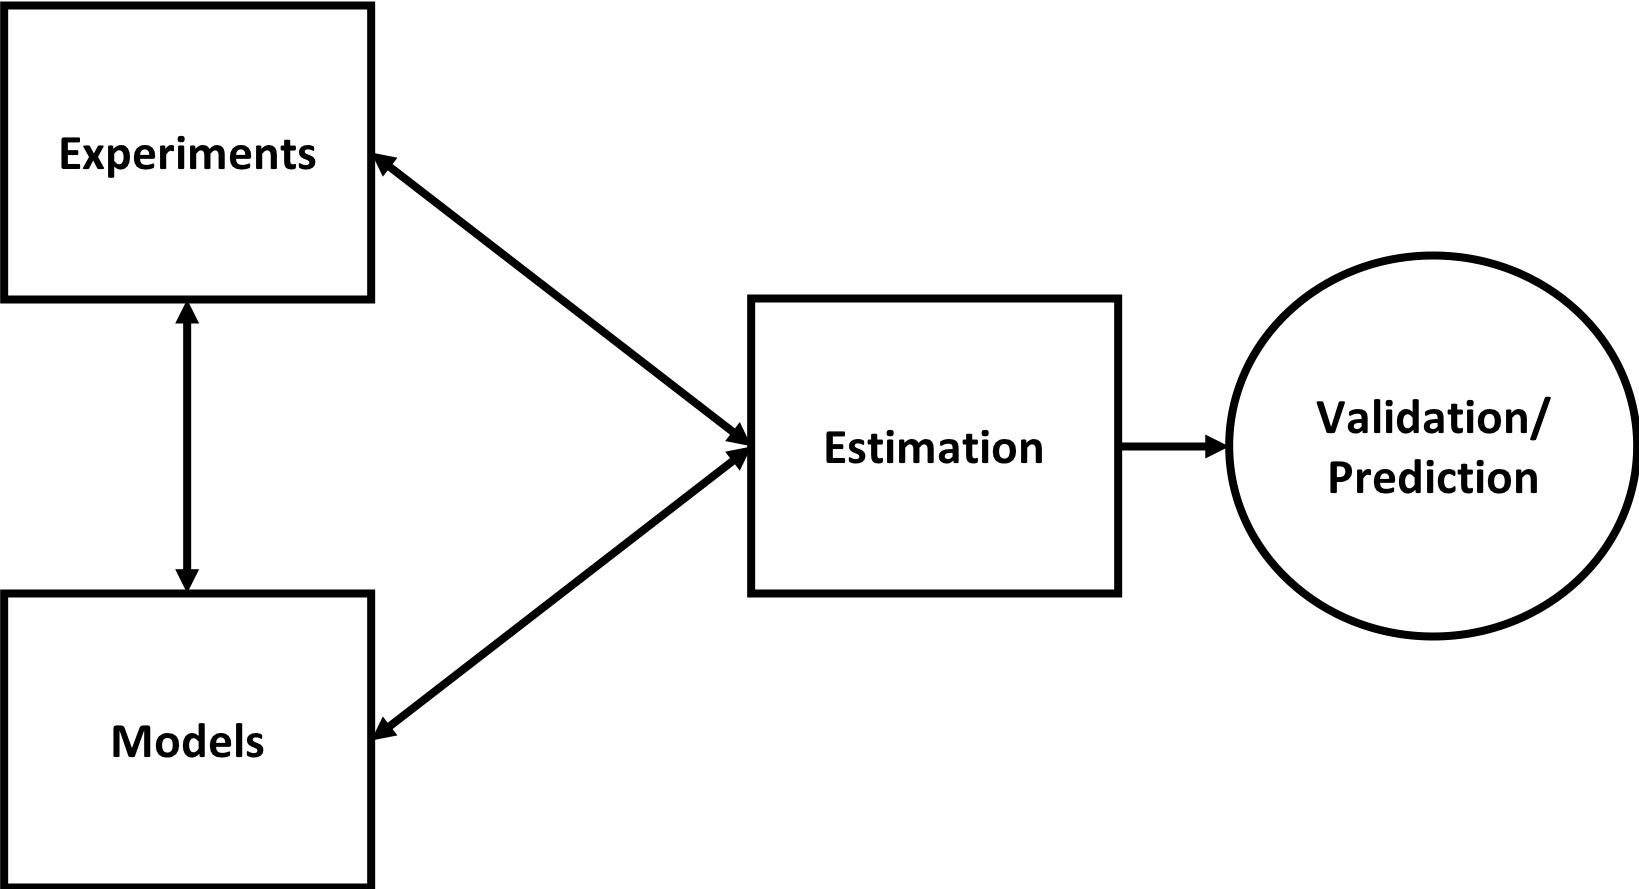
\includegraphics[width=\linewidth]{Chapter1/bockdiagrams.png}
    \caption{Block diagram that illustrates the interaction between modeling, experimentation, and state/parameter estimation for validation/prediction in this thesis.}\label{block_diagram}
%\end{minipage}%
\end{figure}

Electrostatic actuators are classically operated in air. However, impressive work has been done on how they can be operated, and modeled, in the context of electrolytes. The overarching goal of this work is to present electrostatic actuators as viable methods of studying the mechanical properties of cells in biological environments, and for acting as valves, pumps, etc... in a micro-fluidic system. We build on this work in order to create and validate models of electrostatic comb-drive actuators in electrolytes that are quantitatively accurate enough to facilitate precise control of these devices. We find that a purely analytic model is sufficient to describe the behavior of the comb-drive in electrolytes.

\section{Thesis Outline} %Section - 1.2

The remainder of the thesis will proceed as follows:

\begin{itemize}
    \item \textbf{Chapter 2} is split into two general parts. First, we motivate our work by presenting examples of MEMs devices that are used to stretch cells in biological media and in microfluidic systems. Second, we detail the fabrication of the comb-drive actuator devices used in our experiments, and the creation of our experimental apparatus.
    \item \textbf{Chapter 3} describes previously developed lump circuit models for the electrostatic comb-drive in electrolytes, presents our novel models for this context, and outlines the method by which we fit the parameters of these models to collected data.
    \item \textbf{Chapter 4} describes our experimental design, and presents the results of our validation process on lumped circuit models. It describes how well the models fit the data, as well as describes the parameters found by the estimation process.
    \item \textbf{Chapter 5} gives a background on accounting for geometry when modeling inter-digitated actuators, of which comb-drives are a subclass. It then describes a novel model for accounting for the geometry of the comb-drive actuator in electrolytes, and compares the geometric models to the lumped circuit model.
    \item \textbf{Chapter 6} describes the current difficulties of actuating the comb-drive actuator at the frequencies required to obtain full actuation in high concentration electrolytes. We present a promising method for facilitating this, and the current results of this method.
    \item \textbf{Chapter 7} summarizes the thesis, and gives directions for future work.
\end{itemize}

 
\nomenclature[z-DEM]{DEM}{Discrete Element Method}
\nomenclature[z-FEM]{FEM}{Finite Element Method}
\nomenclature[z-PFEM]{PFEM}{Particle Finite Element Method}
\nomenclature[z-FVM]{FVM}{Finite Volume Method}
\nomenclature[z-BEM]{BEM}{Boundary Element Method}
\nomenclature[z-MPM]{MPM}{Material Point Method}
\nomenclature[z-LBM]{LBM}{Lattice Boltzmann Method}
\nomenclature[z-MRT]{MRT}{Multi-Relaxation 
Time}
\nomenclature[z-RVE]{RVE}{Representative Elemental Volume}
\nomenclature[z-GPU]{GPU}{Graphics Processing Unit}
\nomenclature[z-SH]{SH}{Savage Hutter}
\nomenclature[z-CFD]{CFD}{Computational Fluid Dynamics}
\nomenclature[z-LES]{LES}{Large Eddy Simulation}
\nomenclature[z-FLOP]{FLOP}{Floating Point Operations}
\nomenclature[z-ALU]{ALU}{Arithmetic Logic Unit}
\nomenclature[z-FPU]{FPU}{Floating Point Unit}
\nomenclature[z-SM]{SM}{Streaming Multiprocessors}
\nomenclature[z-PCI]{PCI}{Peripheral Component Interconnect}
\nomenclature[z-CK]{CK}{Carman - Kozeny}
\nomenclature[z-CD]{CD}{Contact Dynamics}
\nomenclature[z-DNS]{DNS}{Direct Numerical Simulation}
\nomenclature[z-EFG]{EFG}{Element-Free Galerkin}
\nomenclature[z-PIC]{PIC}{Particle-in-cell}
\nomenclature[z-USF]{USF}{Update Stress First}
\nomenclature[z-USL]{USL}{Update Stress Last}
\nomenclature[s-crit]{crit}{Critical state}
\nomenclature[z-DKT]{DKT}{Draft Kiss Tumble}
\nomenclature[z-PPC]{PPC}{Particles per cell}